\documentclass[11pt]{article}
\usepackage[a4paper,margin=1in]{geometry}
\usepackage{amsmath,amssymb,mathtools}
\usepackage{xcolor}
\usepackage{tikz}
\usepackage{microtype}

\title{Showing that \(\displaystyle \inf_{n\in\mathbb{Z}} \big\{ \frac{n^2+1}{2n-1}\big\} =-\infty\) }
\date{}
\begin{document}
\maketitle

\section*{Intuition}

Consider the function
\[
f:\mathbb{R}\to \mathbb{R}, \quad f(x)=\frac{x^2+1}{2x-1}.
\]
For large positive \(x\), dividing numerator and denominator by \(x\) gives
\[
f(x)=\frac{x+\frac{1}{x}}{2-\frac{1}{x}} \approx \frac{x}{2},
\]
so \(f(x)\), when $|x|$ is large, behaves like the line \(y=\tfrac12 x\). As \(x\to -\infty\), both \(x\) and \(2x-1\) are negative, so the same asymptotic holds:
\[
f(x)\approx \frac{1}{2}x.
\]
The line \(y=\tfrac12 x\) has a steeper (more negative) slope than \(y=\tfrac13 x\) or \(y=\tfrac14 x\):
\[
\tfrac12x < \tfrac13x < \tfrac14x\quad\text{for large negative }x.
\]
Hence, for large negative \(x\), the graph of \(y=\tfrac12x\) lies \emph{below} those of \(y=\tfrac13x\) and \(y=\tfrac14x\), and therefore \(f(x)\) will eventually fall below any of them.
This geometric picture explains why, for any real \(r\), we can find \(n_1\in\mathbb{Z}_{-}\) such that
\[
f(n_1) < \tfrac13 n_1 < r,
\]
so \(\inf f(n)=-\infty.\) (I we can use any of $1/3x$ or $1/4 x$ or a lot of different lines for an easy comparison.)

\begin{center}
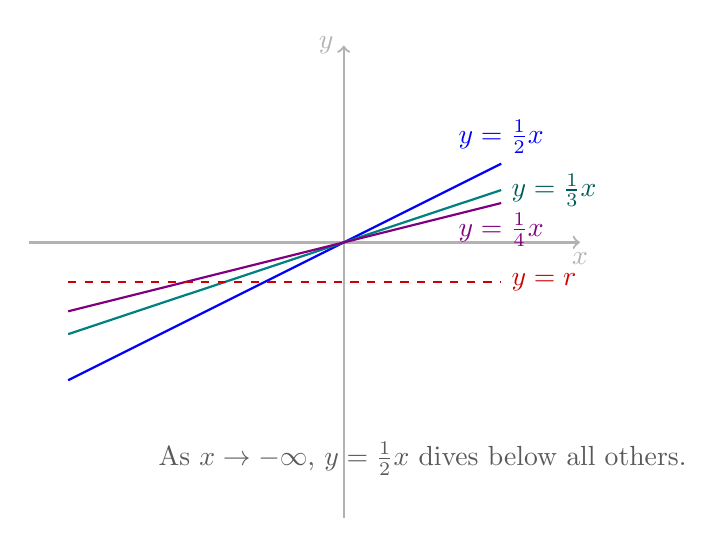
\begin{tikzpicture}[scale=0.5]
  % Axes
  \draw[->, thick, gray!60] (-8,0)--(6,0) node[below]{$x$};
  \draw[->, thick, gray!60] (0,-7)--(0,5) node[left]{$y$};

  % Lines
  \draw[thick, blue] (-7,-3.5)--(4,2) node[above, blue]{$y=\tfrac12x$};
  \draw[thick, teal] (-7,-2.33)--(4,1.33) node[right, teal!70!black]{$y=\tfrac13x$};
  \draw[thick, violet] (-7,-1.75)--(4,1) node[below, violet]{$y=\tfrac14x$};
  \draw[thick, red!80!black, dashed] (-7,-1)--(4,-1) node[right, red!80!black]{$y=r$};

  % Labels and note
  \node[gray!70!black] at (2,-5.5) {As $x\to -\infty$, $y=\tfrac12x$ dives below all others.};
\end{tikzpicture}
\end{center}

\bigskip

\section*{Formal Argument}

For \(n\le 0\), the denominator \(2n-1<0\). Compute:
\[
f(n)-\frac{n}{3}
=\frac{(n^2+1)-\frac{n}{3}(2n-1)}{2n-1}
=\frac{\tfrac13(n^2+n+3)}{2n-1}.
\]
The numerator \(\tfrac13(n^2+n+3)>0\) for when $|n|$ is very large (positive or negative), while the denominator \(2n-1<0\) for \(n\le0\).
Thus
\[
\boxed{f(n)\le \frac{n}{3}\quad\text{for all }n\le0.}
\]

Now let \(r\in\mathbb{R}\).
By the Archimedean property, there exists a negative integer \(n_1\) such that \(\tfrac{n_1}{3}<r\).
Then \(f(n_1)\le\tfrac{n_1}{3}<r\), proving that \(f(n)\) takes values smaller than any real number \(r\).

\[
\boxed{\inf_{n\in\mathbb{Z}} f(n)=-\infty.}
\]

\vskip 2mm
\textbf{Question.}
Can you use a similar argument to show that $\sup_{n\in\mathbb{Z}} \big\{ \frac{n^2+1}{2n-1}\big\} =+\infty?$
\end{document}
